\documentclass[aspectratio=169,
hyperref={colorlinks,urlcolor=blue}
]{beamer}


%\usetheme{Pittsburgh}
\usetheme{default}
\usepackage{colortbl}%colored tables
%For using helvetica font:
\usepackage[scaled]{helvet}
\usepackage[T1]{fontenc}
\renewcommand\familydefault{\sfdefault}
\urlstyle{same} %sets the fonts for urls
\usepackage{pdfpages}
\usepackage{siunitx}
\usepackage{caption}
\usepackage{pifont}%for dings
\usepackage{pgfplots}%for 3d plotting
\pgfplotsset{compat = newest}
\usepackage{mathtools}%box in align env \Aboxed
\usepackage[american,smartlabels]{circuitikz}%for drawing circuits
\usepackage{multimedia}
\usepackage{animate}
\usepackage{xcolor}


\usetikzlibrary{arrows}
\usetikzlibrary {3d} 
\usetikzlibrary{decorations.markings, math}
\usetikzlibrary{intersections, pgfplots.fillbetween}
\usetikzlibrary {shapes.geometric} 


%\definecolor{myblue}{RGB}{5, 34, 150}
\definecolor{myblue2}{RGB}{5, 34, 150}
\definecolor{myblue}{RGB}{0,36,82}
\definecolor{myred}{RGB}{207, 2, 13}
\definecolor{mygreen}{RGB}{0, 158, 11}
\definecolor{myyellow}{RGB}{220,220,0}
\definecolor{qblue}{RGB}{0,36,82}
\definecolor{qgold}{RGB}{250,189,15}
\definecolor{qred}{RGB}{185,14,49}
\definecolor{cblue}{rgb}{0.13, 0.67, 0.8}
\definecolor{corange}{rgb}{0.8, 0.34, 0.0}
\definecolor{cpurple}{rgb}{0.54, 0.29, 0.42}

%%%%%%%%%%%% General settings
\setbeamercolor{frametitle}{fg=black}
\setbeamercolor{title}{fg=black}
\setbeamercolor{author}{fg=myblue2}

\beamertemplatenavigationsymbolsempty %no navigation controls at bottom of slides
%\setbeamertemplate{footline}[frame number]
\usefonttheme{professionalfonts} 
\setbeamerfont{title}{series=\bfseries,parent=structure}
\setbeamerfont{frametitle}{series=\bfseries,parent=structure}

%%%%%%%%%%%%Lists
\setbeamertemplate{itemize item}[circle] %{\color{myblue}$\circ$}
\setbeamertemplate{itemize subitem}{\color{myblue2}$\circ$}
\setbeamertemplate{itemize subsubitem}{\color{myblue2}$\cdot$}
\setbeamercolor{itemize item}{bg=myblue2,fg=myblue2}
\setbeamercolor{enumerate item}{bg=myblue2,fg=myblue2}
%%%%%%%%%%%%%%%%%%%%%%%%%%%%

%%%%%%%%%%%%Blocks
\setbeamertemplate{blocks}[rounded]
%Default block
\setbeamercolor{block title}{bg=myblue2, fg=white}
\setbeamercolor{block body}{bg=myblue2!10}
\setbeamerfont{block body}{size=\scriptsize}
\setbeamerfont{block title}{size=\scriptsize}
%Alert block
\setbeamercolor{block title alerted}{bg= myblue2, fg=white}
\setbeamercolor{block body alerted}{bg=myblue2!10}
\setbeamerfont{block body alerted}{size=\scriptsize}
\setbeamerfont{block title alerted}{size=\scriptsize}
%example block
\setbeamercolor{block title example}{bg=mygreen, fg=white}
\setbeamercolor{block body example}{bg=mygreen!10}
\setbeamerfont{block body example}{size=\scriptsize}
\setbeamerfont{block title example}{size=\scriptsize}
%%%%%%%%%%%%%%%%55


%%%%%%%%%%%%Figures and captions
\captionsetup{font=scriptsize,labelfont=scriptsize}
%\setbeamertemplate{caption}{\raggedright\insertcaption\par}
\newenvironment{capfig}[3]{\begin{figure}\includegraphics[width=#1\textwidth]{#2}\caption*{\textit{#3}}\end{figure}}{}

%\makeatother
%\setbeamertemplate{footline}
%{
%  \leavevmode%
%  \hbox{%
%  \begin{beamercolorbox}[wd=.4\paperwidth,ht=2.25ex,dp=1ex,center]{author in head/foot}%
%    \usebeamerfont{author in head/foot}\insertshortauthor
%  \end{beamercolorbox}%
%  \begin{beamercolorbox}[wd=.6\paperwidth,ht=2.25ex,dp=1ex,center]{title in head/foot}%
%    \usebeamerfont{title in head/foot}\insertshorttitle\hspace*{3em}
%    \insertframenumber{} / \inserttotalframenumber\hspace*{1ex}
%  \end{beamercolorbox}
%  }%
%  \vskip0pt%
%}
%\makeatletter

\makeatother
\setbeamertemplate{footline}
{
  \leavevmode%
  \hbox{%
\begin{beamercolorbox}[wd=.27\paperwidth,ht=2.25ex,dp=1ex,center]{author in head/foot}%
    \color{black}{\insertinstitute}
\end{beamercolorbox}
  \begin{beamercolorbox}[wd=.27\paperwidth,ht=2.25ex,dp=1ex,center]{author in head/foot}%
    \color{black}{\inserttitle}
  \end{beamercolorbox}%
  \begin{beamercolorbox}[wd=.27\paperwidth,ht=2.25ex,dp=1ex,center]{title in head/foot}%
    \color{black}{\insertshortauthor}
  \end{beamercolorbox}
  \begin{beamercolorbox}[wd=.27\paperwidth,ht=2.25ex,dp=1ex,center]{title in head/foot}%
    \hspace{.28\paperwidth}\color{black} \insertframenumber{} / \inserttotalframenumber\hspace*{1ex}
  \end{beamercolorbox}
  }%
  \vskip0pt%
}
\makeatletter

\setbeamertemplate{title page}
{
  \begin{tikzpicture}[remember picture,overlay]
    \def\barh{4}%15
  
    \draw[color=myblue2,line width=\barh] ([yshift=-0.5*\barh]current page.north west) -- ([yshift=-0.5*\barh,xshift=-0.67\paperwidth]current page.north east);
    \draw[color=myblue2,line width=\barh] ([yshift=-0.5*\barh,xshift=-0.67\paperwidth]current page.north east) -- ([yshift=-0.5*\barh,xshift=-0.34\paperwidth]current page.north east);
    \draw[color=myblue2,line width=\barh] ([yshift=-0.5*\barh,xshift=-0.34\paperwidth]current page.north east) -- ([yshift=-0.5*\barh]current page.north east); 
  
    \draw[color=myblue2,line width=\barh] ([yshift=0.5*\barh]current page.south west) -- ([yshift=0.5*\barh,xshift=-0.67\paperwidth]current page.south east);
    \draw[color=myblue2,line width=\barh] ([yshift=0.5*\barh,xshift=-0.67\paperwidth]current page.south east) -- ([yshift=0.5*\barh,xshift=-0.34\paperwidth]current page.south east);
    \draw[color=myblue2,line width=\barh] ([yshift=0.5*\barh,xshift=-0.34\paperwidth]current page.south east) -- ([yshift=0.5*\barh]current page.south east);
    %\node[left] at (current page.east) {
    %
\includegraphics[scale=0.1]{figures/coverpage}
    %};
  \end{tikzpicture}
  
  \usebeamerfont{title}\usebeamercolor[fg]{title}\inserttitle\par
  \usebeamerfont{subtitle}\usebeamercolor[fg]{subtitle}\insertsubtitle\par
  \vspace{2cm}
  \usebeamerfont{author}\usebeamercolor[fg]{author}\insertauthor\par
  \usebeamerfont{institute}\usebeamercolor[fg]{author}\insertinstitute\par
  \usebeamercolor[fg]{author}\par
  \usebeamercolor[fg]{titlegraphic}\inserttitlegraphic

} 

\setbeamertemplate{frametitle}{%
    \nointerlineskip%
        \par\hspace*{-\dimexpr0.5\paperwidth-0.5\textwidth}\textcolor{myblue2}{\rule{0.33\paperwidth}{6pt}}\textcolor{myblue2}{\rule{0.33\paperwidth}{6pt}}\textcolor{myblue2}{\rule{0.34\paperwidth}{6pt}} 
    \begin{beamercolorbox}[wd=\paperwidth,ht=0.75cm,dp=0.6ex]{frametitle}
        \hspace*{0.5cm}\strut\usebeamerfont{frametitle}\insertframetitle\strut
        %\hrule
    \end{beamercolorbox}%
    %%Line below:
%\par\hspace*{-\dimexpr0.5\paperwidth-0.5\textwidth}\textcolor{myblue}{\rule{\paperwidth}{0.4pt}}
     % <-- calculation of left margin width + rule
     %\textcolor{red}{\noindent\rule{\paperwidth}{2pt}}
}


%%%%%%%%%%%%Frame templates

%Slide with title
\newenvironment{titleframe}[1]
{\begin{frame}\frametitle{#1}\end{frame}}
{}

%Slide with title and itemize list:
\newenvironment{bulletframe}[1]
{\begin{frame}{#1} \itemize}
{\enditemize \end{frame}}

%Slide with two columns 50/50
\newenvironment{twocolframe}[3]
{\begin{frame}{#1}
 \begin{columns}[T]
 \column{0.5\textwidth}#2
 \column{0.5\textwidth}#3
 \end{columns}\end{frame}}{}

%Slide with two columns 60/40 <<<<<<<<<<<<<<<<<<<<<<  This one!
\newenvironment{twocolframesf}[3]
{\begin{frame}{#1}
 \begin{columns}[T]
 \column{0.6\textwidth}#2
 \column{0.4\textwidth}#3
 \end{columns}\end{frame}}{}
 
%Slide with two columns 70/30
\newenvironment{twocolframest}[3]
{\begin{frame}{#1}
 \begin{columns}[T] 
 \column{0.7\textwidth}#2
 \column{0.3\textwidth}#3
 \end{columns}\end{frame}}{} 
 
%Slide with two columns 40/60
\newenvironment{twocolframefs}[3]
{\begin{frame}{#1}
 \begin{columns}[T] 
 \column{0.4\textwidth}#2
 \column{0.6\textwidth}#3
 \end{columns}\end{frame}}{}
 
%Slide with two columns 70/30
\newenvironment{twocolframets}[3]
{\begin{frame}{#1}
 \begin{columns}[T] 
 \column{0.3\textwidth}#2
 \column{0.7\textwidth}#3
 \end{columns}\end{frame}}{} 

 
%Colloquium speaker (title, abstract, picture file, speaker name)
\newenvironment{colloquium}[5]
{
\begin{frame}{Colloquium: Friday 1:30pm in Stirling A}
\begin{columns}[T] 
 \column{0.8\textwidth}
 \textbf{#1}\\
 #2
 \column{0.2\textwidth}
 \capfig{#3}{#4}{#5}
 \end{columns}
\end{frame}
}
{} 

%%%%%%%%%%%%%Set Hyperref colors


\hypersetup{
  colorlinks=true,
  linkcolor=blue,    
  urlcolor=blue,     
  citecolor=blue      
}
%%%%%%%%%%%%%TOC bolding
\setbeamerfont{section in toc}{series=\bfseries}



%Frames:
% \twocolframesf 60/40 (fs, st, ts) 
% \titleframe
% bulletframe


%%%%%%%%%%%%%%%%%%%%%%%%%
%%%%%% START OF PRESENTATION %%%%%%
%%%%%%%%%%%%%%%%%%%%%%%%%
\title{Circuits}
\subject{Modeling and Solving Circuits, and Kirchoff's Laws}
\subtitle{Building Models to Describe our World}


%%%%%%%%%%%%%%%%%%%%%%%%%%%%%%
%%%%%%%%%%%%%%%%%%%%%



\begin{document}

%%%%%%%%%%%%%%%%%%%%%%%%%
%%%%%% Title slide %%%%%%
%%%%%%%%%%%%%%%%%%%%%%%%%
\chaptertitle{Circuits}
\begin{frame}
\titlepage
\thispagestyle{empty}

\begin{textblock*}{5cm}(11cm,4cm)
    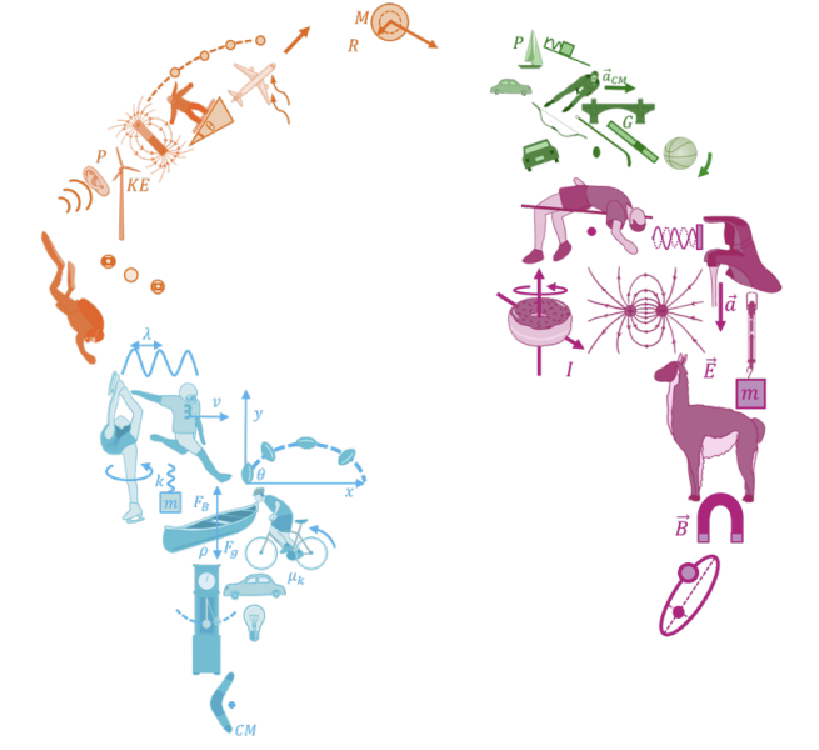
\includegraphics[width=4cm]{figures/BMDW/logo}
\end{textblock*}

\end{frame}

%%%%%%%%%%%%%TOC
\twocolframe{Outline}
  {\tableofcontents[sections={1,2}, subsectionstyle=show/show]\thispagestyle{empty}}
  {\tableofcontents[sections={3}, subsectionstyle=show/show]}
%%%%%%%%%%%%%%%%%%%%%%%%%







%%%%%%%%%%%%%%%%%%%%%%%%%%%%%%%%
\section{Modeling Circuits}
\label{sec:modelingcircuits}
\title{Modeling Circuits}


%%%%%%%%%%%%%%%%%%%%%%%%%
\begin{frame}
\titlepage
\thispagestyle{empty}
\end{frame}


%%%%%%%%%%%%%%%%%%%%%%%%



\def\proton at (#1,#2,#3){
\draw[fill=black,opacity=1] (#1,#2) circle (#3);
% a plus sign that scales
\draw[color=white] (#1-0.8*#3,#2) -- (#1+0.8*#3,#2);
\draw[color=white] (#1,#2-0.8*#3) -- (#1,#2+0.8*#3);
}

\def\ion at (#1,#2,#3){
\draw[fill=orange,opacity=1,draw=orange] (#1,#2) circle (#3);
% a plus sign that scales
\draw[color=white] (#1-0.8*#3,#2) -- (#1+0.8*#3,#2);
\draw[color=white] (#1,#2-0.8*#3) -- (#1,#2+0.8*#3);
}

\def\electron at (#1,#2,#3){
\fill[color=myred,opacity=1] (#1,#2) circle (#3);
% a minus sign that scales
\draw[color=white] (#1-0.8*#3,#2) -- (#1+0.8*#3,#2);
}

%%%%%%%%%%%%%%%%%%%%%%%%%%%%%%
\subsection{The electric cell}
\label{subsec:thelectriccell}
\twocolframe{The electric cell}
{
\begin{itemize}
\item Zinc ``likes'' to be dissolved as an ion in acid.
\item The zinc ions leave their electrons behind in the electrode, making the zinc electrode negatively charged.
\item Electrons that are loosely bound in a carbon electrode are attracted into the electrolyte solution, leaving the carbon electrode positively charged.
\item Very quickly, the process stops as an equilibrium is reached, with a net electric potential difference between electrodes.
\end{itemize}
}
{ 
\begin{center}

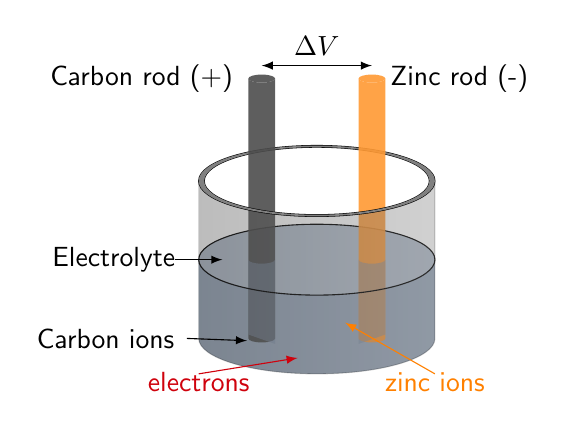
\begin{tikzpicture}[scale=1]
\tikzmath{
\Lou=2.0;
\Lw=1.0;
\Rou=1.5;
\dr=0.07;
\fac=0.3;
\Rd=0.17;
\Ld=3.3;
\xs=0.7;
\rp=0.1;
\re=0.05;
}  

\scalebox{1}{
%liquid:
  \fill[color=myblue!80,opacity=0.5] (-\Rou,0) arc (180:360:{\Rou} and {\fac*\Rou}) --  (\Rou,0)-- (\Rou, \Lw) arc (0:-180:{\Rou} and {\fac*\Rou}) -- (-\Rou,\Lw); 
  \fill[color=myblue!60, opacity=0.5] (\Rou,\Lw) arc (0:360:{\Rou} and {\fac*\Rou}) ;
 \draw[color=black] (\Rou,\Lw) arc (0:180:{\Rou} and {\fac*\Rou}) ;

%BACK RIM OF CONTAINER
  \draw[color=myblue!50, color=black, opacity=1, name path=A1] (\Rou,\Lou) arc (0:180:{\Rou} and {\fac*\Rou}) ;
  \draw[color=myblue!20, color=black, opacity=1, name path=B1] (\Rou-\dr,\Lou) arc (0:180:{\Rou-\dr} and {\fac*(\Rou-\dr)});
  \tikzfillbetween[of=A1 and B1]{gray}; 
  
%Rods:
  \fill[color=black!70,opacity=0.9] (-\Rd-\xs,0) arc (180:360:{\Rd} and {\fac*\Rd}) --  (\Rd-\xs,0)-- (\Rd-\xs, \Ld) arc (0:-180:{\Rd} and {\fac*\Rd}) -- (-\Rd-\xs,\Ld); 
  \fill[color=black!70, opacity=0.9] (\Rd-\xs,\Ld) arc (0:360:{\Rd} and {\fac*\Rd}) ;
  %\draw[color=black, dashed] (\Rd-\xs,\Lw) arc (0:360:{\Rd} and {\fac*\Rd}) ;
  \fill[color=myblue!50, opacity=0.5] (\Rd-\xs,\Lw) arc (0:-180:{\Rd} and {\fac*\Rd})  -- (-\xs-\Rd,\Lw-0.95) -- (-\xs+\Rd,\Lw-1.07);
    
  \fill[color=orange!80, opacity=0.9] (-\Rd+\xs,0) arc (180:360:{\Rd} and {\fac*\Rd}) --  (\Rd+\xs,0)-- (\Rd+\xs, \Ld) arc (0:-180:{\Rd} and {\fac*\Rd}) -- (-\Rd+\xs,\Ld); 
  \fill[color=orange!80, opacity=0.9] (\Rd+\xs,\Ld) arc (0:360:{\Rd} and {\fac*\Rd}) ;
  %\draw[color=orange, dashed] (\Rd+\xs,\Lw) arc (0:360:{\Rd} and {\fac*\Rd}) ;
  \fill[color=myblue!50, opacity=0.5] (\Rd+\xs,\Lw) arc (0:-180:{\Rd} and {\fac*\Rd})-- (\xs-\Rd,\Lw-1.07)  -- (\xs+\Rd,\Lw-0.95) ;
   
  \draw[color=black] (\Rou,\Lw) arc (0:-180:{\Rou} and {\fac*\Rou}) ;
   
%% particles
  \foreach \i in {1,3,...,7} {
   \proton at (-\xs-0.05,\i*\Ld/7-0.5,1.1*\rp)
   \electron at (\xs-0.07,\i*\Ld/7-0.5,1.1*\re)
  } 
  \foreach \i in {2,4,...,7} {
   \proton at (-\xs+0.07,\i*\Ld/7-0.5,0.9*\rp)
   \electron at (\xs+0.07,\i*\Ld/7-0.5,0.9*\re)
  } 
  
  \ion at (\xs-1.8*\Rd,1.3,0.9*\rp)
  \ion at (\xs-3*\Rd,1.2,0.9*\rp)
  \ion at (\xs-2*\Rd,\Ld/7-0.5,0.9*\rp)
  \ion at (\xs-2*\Rd,0.2,0.9*\rp)
  \ion at (\xs-3.2*\Rd,\Ld/7-0.7,\rp)
  \ion at (\xs-4*\Rd,0,1.1*\rp)
  \ion at (\xs-4.5*\Rd,\Ld/7-0.5,1.1*\rp)
  
  \electron at (-\xs+1.2*\Rd,\Ld/7-0.5,0.9*\re)
  \electron at (-\xs+2*\Rd,0.2,0.9*\re)
  \electron at (-\xs+2*\Rd,0.6,0.9*\re)
  \electron at (-\xs+1.7*\Rd,1.2,1.1*\re)
  \electron at (-\xs+2.8*\Rd,\Ld/7-0.7,\re)
  \electron at (-\xs+3*\Rd,0.4,1.1*\re)
  \electron at (-\xs+2.5*\Rd,\Ld/7,\re)
          
%front of container:
  \fill[left color=gray,right color=gray!20,shading=axis,opacity=0.2, draw=black] (-\Rou,0) arc (180:360:{\Rou} and {\fac*\Rou}) --  (\Rou,0)-- (\Rou, \Lou) arc (0:-180:{\Rou} and {\fac*\Rou}) -- (-\Rou,\Lou); 
  \draw[color=myblue!50, color=black, opacity=1, name path=A2] (\Rou,\Lou) arc (0:-180:{\Rou} and {\fac*\Rou}) ;
  \draw[color=myblue!20, color=black, opacity=1, name path=B2] (\Rou-\dr,\Lou) arc (0:-180:{\Rou-\dr} and {\fac*(\Rou-\dr)});
  \tikzfillbetween[of=A2 and B2]{gray}; 
 
 
 \node[above, left=2pt] at (-\Rd-\xs,\Ld){{Carbon rod (+)}};
 \node[above, right=8pt] at (-\Rd+\xs,\Ld){{Zinc rod (-)}};
 \draw[color=myred,-latex](-\Rou,-0.6*\Rou/2)  node[below=-4pt] {{electrons}}  -- (-\xs+2.8*\Rd,\Ld/7-0.7,\re);
 \draw[-latex](-1.1*\Rou,0)  node[left=1pt] {{Carbon ions}}  -- (-\xs-1.1*\Rd,\Ld/7-0.5);
 \draw[color=orange,-latex](\Rou,-0.6*\Rou/2)  node[below=-4pt] {{zinc ions}}  -- (\xs-2*\Rd,0.2);
 \draw[-latex] (-1.2*\Rou,\Lou/2) -- (-0.8*\Rou,\Lou/2);
 \node[left=5pt] at (-\Rou,\Lou/2) {{Electrolyte}};  
 \draw[latex-latex] (-\xs,1.05*\Ld) -- (\xs,1.05*\Ld) node[above,midway] {{$\Delta V$}}; 
 }
\end{tikzpicture}
\captionof*{figure}{\textit{An electric cell made with an electrolyte, such as $H_2SO_4$ (sulfuric acid) and two metals.}}
\end{center}
}


%%%%%%%%%%%%%%%%%%%%%%%%%%%%%%



%%%%%%%%%%%%%%%%%%%%%%%%%%%%%%
\subsection{Current flow in a battery}
\label{subsec:currentflowinabattery}
\twocolframesf{Current flow in a battery}
{
\begin{itemize}
\item The rate of chemical reactions in the battery limits the current that can be produced. 
\item The components of the battery themselves will have a finite resistance (e.g. the rods). 
\item If the resistance of the resistor (and battery) is low enough, the rate of chemical reactions cannot sustain the current implied by Ohm's Law ($V=RI$). The voltage of the battery thus drops until the current given by Ohm's Law can be sustained by the chemical reactions.
\end{itemize}
}
{
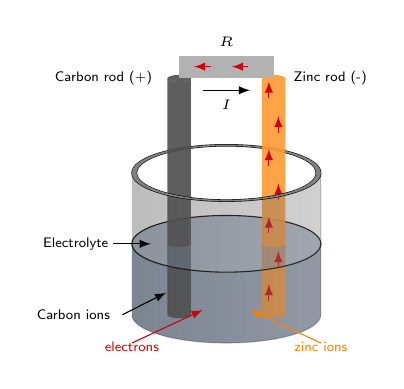
\begin{tikzpicture}[scale=0.3]
  \def\Lou{6.0}
  \def\Lw{3.0}
  \def\Rou{4}
  \def\dr{0.2}
  \def\fac{0.3}
  \def\Rd{0.5}
  \def\Ld{10}
  \def\xs{2}
  \def\rp{0.3}
  \def\re{0.15}
  
%liquid:
  \fill[color=myblue!80,opacity=0.5] (-\Rou,0) arc (180:360:{\Rou} and {\fac*\Rou}) --  (\Rou,0)-- (\Rou, \Lw) arc (0:-180:{\Rou} and {\fac*\Rou}) -- (-\Rou,\Lw); 
  \fill[color=myblue!60, opacity=0.5] (\Rou,\Lw) arc (0:360:{\Rou} and {\fac*\Rou}) ;
 \draw[color=black] (\Rou,\Lw) arc (0:180:{\Rou} and {\fac*\Rou}) ;

%BACK RIM OF CONTAINER
  \draw[color=myblue!50, color=black, opacity=1, name path=A1] (\Rou,\Lou) arc (0:180:{\Rou} and {\fac*\Rou}) ;
  \draw[color=myblue!20, color=black, opacity=1, name path=B1] (\Rou-\dr,\Lou) arc (0:180:{\Rou-\dr} and {\fac*(\Rou-\dr)});
  \tikzfillbetween[of=A1 and B1]{gray}; 
  

%Rods:
  \fill[color=black!70,opacity=0.9] (-\Rd-\xs,0) arc (180:360:{\Rd} and {\fac*\Rd}) --  (\Rd-\xs,0)-- (\Rd-\xs, \Ld) arc (0:-180:{\Rd} and {\fac*\Rd}) -- (-\Rd-\xs,\Ld); 
  \fill[color=black!70, opacity=0.9] (\Rd-\xs,\Ld) arc (0:360:{\Rd} and {\fac*\Rd}) ;
  \fill[color=myblue!50, opacity=0.5] (\Rd-\xs,\Lw) arc (0:-180:{\Rd} and {\fac*\Rd})  -- (-\xs-\Rd,\Lw-0.95) -- (-\xs+\Rd,\Lw-1.07);
    
  \fill[color=orange!80, opacity=0.9] (-\Rd+\xs,0) arc (180:360:{\Rd} and {\fac*\Rd}) --  (\Rd+\xs,0)-- (\Rd+\xs, \Ld) arc (0:-180:{\Rd} and {\fac*\Rd}) -- (-\Rd+\xs,\Ld); 
  \fill[color=orange!80, opacity=0.9] (\Rd+\xs,\Ld) arc (0:360:{\Rd} and {\fac*\Rd}) ;
  \fill[color=myblue!50, opacity=0.5] (\Rd+\xs,\Lw) arc (0:-180:{\Rd} and {\fac*\Rd})-- (\xs-\Rd,\Lw-1.07)  -- (\xs+\Rd,\Lw-0.95) ;
   
  \draw[color=black] (\Rou,\Lw) arc (0:-180:{\Rou} and {\fac*\Rou}) ;
   
%% particles
  \foreach \i in {1,3,...,7} {
   \proton at (-\xs-0.15,\i*\Ld/7-0.5,1.1*\rp)
   \electron at (\xs-0.2,\i*\Ld/7-1,1.1*\re)
   \draw [-latex,color=myred] (\xs-0.2,\i*\Ld/7-1+1.1*\re)--(\xs-0.2,\i*\Ld/7-1+1.1*\re+0.7);
   
  } 
  \foreach \i in {2,4,...,7} {
   \proton at (-\xs+0.2,\i*\Ld/7-0.5,0.9*\rp)
   \electron at (\xs+0.2,\i*\Ld/7-1,0.9*\re)
   \draw [-latex,color=myred] (\xs+0.2,\i*\Ld/7-1+0.9*\re)--(\xs+0.2,\i*\Ld/7-1+0.9*\re+0.7);
  } 
  
  \ion at (\xs-1.8*\Rd,1.3,0.9*\rp)
  \ion at (\xs-3*\Rd,1.2,0.9*\rp)
  \ion at (\xs-2*\Rd,\Ld/7-0.5,0.9*\rp)
  \ion at (\xs-2*\Rd,0.2,0.9*\rp)
  \ion at (\xs-3.2*\Rd,\Ld/7-0.7,\rp)
  \ion at (\xs-4*\Rd,0,1.1*\rp)
  \ion at (\xs-4.5*\Rd,\Ld/7-0.5,1.1*\rp)
  \ion at (\xs-5*\Rd,-0.2,1.1*\rp)
  \ion at (\xs-2.7*\Rd,0,\rp)
  
  \electron at (-\xs+1.2*\Rd,\Ld/7-0.5,0.9*\re)
  \electron at (-\xs+2*\Rd,0.2,0.9*\re)
  \electron at (-\xs+2*\Rd,0.6,0.9*\re)
  \electron at (-\xs+1.7*\Rd,1.2,1.1*\re)
  \electron at (-\xs+2.8*\Rd,\Ld/7-0.7,\re)
  \electron at (-\xs+3*\Rd,0.4,1.1*\re)
  \electron at (-\xs+2.5*\Rd,\Ld/7,\re)
  %\electron at (-\xs+4*\Rd,0.6,1.1*\re)
  %\electron at (-\xs+3.7*\Rd,1.4,1.1*\re)    
%front of container:
  \fill[left color=gray,right color=gray!20,shading=axis,opacity=0.2, draw=black] (-\Rou,0) arc (180:360:{\Rou} and {\fac*\Rou}) --  (\Rou,0)-- (\Rou, \Lou) arc (0:-180:{\Rou} and {\fac*\Rou}) -- (-\Rou,\Lou); 
  \draw[color=myblue!50, color=black, opacity=1, name path=A2] (\Rou,\Lou) arc (0:-180:{\Rou} and {\fac*\Rou}) ;
  \draw[color=myblue!20, color=black, opacity=1, name path=B2] (\Rou-\dr,\Lou) arc (0:-180:{\Rou-\dr} and {\fac*(\Rou-\dr)});
  \tikzfillbetween[of=A2 and B2]{gray}; 
 
 %resistor
 \draw[line width=8pt,black!30=qred!] (-\xs,1.05*\Ld) -- (\xs,1.05*\Ld) node[above,midway,color=black] {\tiny{$R$}}; 
 \electron at (\xs-1.8*\Rd,1.05*\Ld,1.1*\re)
 \draw [-latex,color=myred] (\xs-1.8*\Rd-1.1*\re,1.05*\Ld) -- (\xs-1.8*\Rd-1.1*\re-0.7,1.05*\Ld);
 \electron at (\xs-5*\Rd,1.05*\Ld,1.1*\re)
 \draw [-latex,color=myred] (\xs-5*\Rd-1.1*\re,1.05*\Ld) -- (\xs-5*\Rd-1.1*\re-0.7,1.05*\Ld);
 
 
 \node[above, left=2pt] at (-\Rd-\xs,\Ld){\tiny{Carbon rod (+)}};
 \node[above, right=8pt] at (-\Rd+\xs,\Ld){\tiny{Zinc rod (-)}};
 \draw[color=myred,-latex](-\Rou,-0.6*\Rou/2)  node[below=-4pt] {\tiny{electrons}}  -- (-\xs+2*\Rd,0.2);
 \draw[-latex](-1.1*\Rou,0)  node[left=1pt] {\tiny{Carbon ions}}  -- (-\xs-1.1*\Rd,\Ld/7-0.5);
 \draw[color=orange,-latex](\Rou,-0.6*\Rou/2)  node[below=-4pt] {\tiny{zinc ions}}  -- (\xs-2*\Rd,0.2);
 \draw[-latex] (-1.2*\Rou,\Lou/2) -- (-0.8*\Rou,\Lou/2);
 \node[left=5pt] at (-\Rou,\Lou/2) {\tiny{Electrolyte}};  
 \draw[-latex] (-0.5*\xs,0.95*\Ld) -- (0.5*\xs,0.95*\Ld) node[midway,below]{\tiny{$I$}};
\end{tikzpicture}
\captionof*{figure}{\textit{As electrons leave the zinc, more ions can dissolve. They eventually neutralize in the solution as electrons come in through the carbon.}}
}



%%%%%%%%%%%%%%%%%%%%%%%%%%%%%%
\subsection{Modeling a real battery}
\label{subsec:modelingarealbattery}
\twocolframesf{Modeling a real battery}
{

\begin{itemize}
\item We can model a real battery as an ideal battery + a resistor (``internal resistance'').
\item The ``emf'', $\epsilon$, is the potential difference of the ideal battery:
\begin{itemize}
 \item It is a constant, independent of what we connect to the battery.
 \item ``Internal voltage'' of the battery, if you prefer a better description than ``electromotive force''.
\end{itemize}
\item The ``terminal voltage'' is the actual voltage measured at the external terminals of the battery. It \textit{depends on the current flowing through the battery} (which results in a voltage drop across the internal resistance, $r$).
\end{itemize}
}
{
\centering
\begin{circuitikz}[scale=0.2]
\def\h{6}
\def\L{20}
\def\w{12}
\def\Rt{1}
\def\fs{0.6}

%rectangular prism
\fill[top color=myred!20,bottom color=myred!80,shading=axis,opacity=0.8, draw=black] (0,0,0) -- (0,\h,0) -- (\L,\h,0) -- (\L, 0, 0); 
\fill[top color=myred!80,bottom color=myred!20,shading=axis,opacity=0.8, draw=black] (0,\h,0) --(0,\h,-\w) -- (\L,\h,-\w) -- (\L, \h, 0); 
\fill[top color=myred!20,bottom color=myred!80,shading=axis,opacity=0.8, draw=black] (\L, 0, 0) --  (\L, \h, 0) -- (\L,\h,-\w) --(\L,0,-\w); 


%battery terminals (by stacking circles!)
\foreach \i in {0,0.05,...,0.5} {
  \begin{scope}[canvas is xz plane at y=\h+\i]
    \fill (0.15*\L,-\w/2) circle(\Rt);
    \fill (0.85*\L,-\w/2) circle(\Rt);
  \end{scope}
}
%circuit components
\scalebox{\fs}{
  \begin{scope}[canvas is xz plane at y=\h/\fs]
    \draw (0.15*\L/\fs,-\w/2/\fs) [short,thick] to (0.3*\L/\fs,-\w/2/\fs)
     to [R,thick] (0.5*\L/\fs,-\w/2/\fs)
     to [battery1={$\,$},thick] (0.7*\L/\fs,-\w/2/\fs)
     to [short,thick] (0.85*\L/\fs,-\w/2/\fs);
  \end{scope}
}

\node[above=-3pt,color=white] at (0.22*\L,\h,0) {\small A};
\node[above=-3pt,color=white] at (0.92*\L,\h,0) {\small B};
\node[above=-3pt] at (0.7*\L+0.25,\h,0) {{\textbf{$\epsilon$}}};
\node[above=-3pt] at (0.5*\L,\h,0) {\small{\textbf{$r$}}};
\draw[latex-latex] (0.28*\L,2*\h) -- (0.95*\L,2*\h) node[above,midway] {\small{Terminal voltage, $V_{AB}$}}; 

\end{circuitikz}
\captionof*{figure}{\textit{A real battery, modelled with an internal resistance.}}
}


%%%%%%%%%%%%%%%%%%%%%%%%%%%%%%



%%%%%%%%%%%%%%%%%%%%%%%%%%%%%%
\subsection{Terminal voltage in a real ciruit}
\label{subsec:terminalvoltageinarealcircuit}
\twocolframesf{Terminal voltage in a real circuit}
{

\begin{itemize}
\item The current through both resistors is \SI{3}{A}.% 
\item The voltage drop across a resistor, $V=RI$:
\begin{itemize}
\item The voltage drop across the \SI{2}{\Omega} resistor is $(\SI{2}{\Omega})(\SI{3}{A})=\SI{6}{V}$
\item The voltage drop across the \SI{1}{\Omega} resistor is $(\SI{1}{\Omega})(\SI{3}{A})=\SI{3}{V}$
\end{itemize}
\item We identify that the “terminal voltage” is between the $-$ terminal ($B$) of the ideal battery, and the point between the two resistors ($A$)
\item The terminal voltage is $V=\SI{9}{V}-\SI{6}{V}=\SI{3}{V}$
\textit{assuming the internal battery can sustain $\SI{3}{A}$}.
\end{itemize}
With a larger resistor, $R$, the total current would be smaller and the voltage drop across $r$ negligible. 
}
{
\vspace{-2cm}
\centering
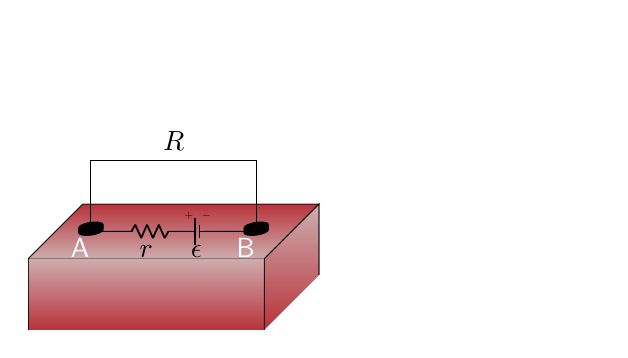
\begin{tikzpicture}[scale=0.15]
\def\h{6}
\def\L{20}
\def\w{12}
\def\Rt{1}
\def\fs{0.4}

%rectangular prism
\fill[top color=myred!20,bottom color=myred!80,shading=axis,opacity=0.8, draw=black] (0,0,0) -- (0,\h,0) -- (\L,\h,0) -- (\L, 0, 0); 
\fill[top color=myred!80,bottom color=myred!20,shading=axis,opacity=0.8, draw=black] (0,\h,0) --(0,\h,-\w) -- (\L,\h,-\w) -- (\L, \h, 0); 
\fill[top color=myred!20,bottom color=myred!80,shading=axis,opacity=0.8, draw=black] (\L, 0, 0) --  (\L, \h, 0) -- (\L,\h,-\w) --(\L,0,-\w); 

%battery terminals (by stacking circles!)
\foreach \i in {0,0.05,...,0.5} {
  \begin{scope}[canvas is xz plane at y=\h+\i]
    \fill (0.15*\L,-\w/2) circle(\Rt);
    \fill (0.85*\L,-\w/2) circle(\Rt);
  \end{scope}
}
%circuit components
\scalebox{\fs}{
  \begin{scope}[canvas is xz plane at y=\h/\fs]
    \draw (0.15*\L/\fs,-\w/2/\fs) [short,thick] to (0.3*\L/\fs,-\w/2/\fs)
     to [R,thick] (0.5*\L/\fs,-\w/2/\fs)
     to [battery1={$\,$},thick] (0.7*\L/\fs,-\w/2/\fs)
     to [short,thick] (0.85*\L/\fs,-\w/2/\fs);
  \end{scope}
}

%wire
\draw[] (0.15*\L,\h,-\w/2) -- (0.15*\L,2.*\h,-\w/2) -- (0.85*\L,2.*\h,-\w/2) node[midway, above] {$R$} -- (0.85*\L,\h,-\w/2);

\node[above=-3pt,color=white] at (0.22*\L,\h,0) {A};
\node[above=-3pt,color=white] at (0.92*\L,\h,0) {B};
\node[above=-3pt] at (0.7*\L+0.25,\h,0) {{\textbf{$\epsilon$}}};
\node[above=-3pt] at (0.5*\L,\h,0) {{\textbf{$r$}}};

\end{tikzpicture}%

\captionof*{figure}{\textit{A battery shorted with a wire of resistance, $R$}}%

\vspace{-0.7cm}
\begin{circuitikz}
\scalebox{0.85}
{
\def\h{2}
\def\L{4}

 \draw (0,0)  [battery1={$\,$},l^=$\epsilon$,-*,i=$I$] to (\L,0) node[below] {B};
 \draw (\L,0) [short] to (\L,\h)
       to [R,l_=$R\;(\SI{1}{\Omega})$,-*] (0.5*\L,\h) node[above] {A}
       to [R,l_=$r\;(\SI{2}{\Omega})$,] (0,\h)
       to [short] (0,0);
       
 \node[color=myred] at (0.25*\L,0.75*\h) {$\SI{6}{V}$};
 \node[color=myred] at (0.5*\L,0.75*\h) {$+$};
 \node[color=myred] at (0.75*\L,0.75*\h) {$\SI{3}{V}$};
 \node[color=myred] at (0.5*\L,-0.3*\h) {$\SI{9}{V}$};
}
\end{circuitikz}%
\captionof*{figure}{\textit{Circuit diagram for the shorted battery. The current is $I=\frac{\SI{9}{V}}{(\SI{2}{\Omega})+(\SI{4}{\Omega})}=\SI{3}{A}$}}%
}


%%%%%%%%%%%%%%%%%%%%%%%%%%%%%%



%%%%%%%%%%%%%%%%%%%%%%%%%%%%%%
\subsection{Analysing ciruits}
\label{subsec:analysingciruits}
\twocolframe{Analysing circuits}
{
\begin{itemize}
\item  If you know the currents through all of the resistors in a circuit, you know everything that there is to know about the circuit:
\begin{itemize}
\item  Given the currents in all resistors, you can calculate the voltage across each of the resistors.
\end{itemize}
\item  Usually, the easiest method to do this is to combine resistors together into equivalent resistors.
\item  However, this cannot always be done, in particular, when the circuit contains more than one battery.
\end{itemize}
}
{\begin{circuitikz}[scale=0.7]
\scalebox{1}
{
\def\h{2}
\def\L{4}

 \draw (-\L,0) node[below] {f}   [battery1,l_={$V_1=\SI{24}{V}$},*-*] to (0,0);
 \draw (-\L,0) to [short,-*] (-\L,\L) node[above] {a}
       to [R,l_={$R_1=\SI{3}{\Omega}$},-*] (0,\L) node[above] {b}
       to [R,l_={$R_2=\SI{3}{\Omega}$}] (0,0) node[below] {e} ;
 \draw (0,0)  [battery1,l_={$V_2=\SI{29}{V}$},*-,invert] to (\L,0) node[below] {d};
 \draw (\L,0) to [R,l^={$R_4=\SI{4}{\Omega}$},-*]  (\L,\L) node[above] {c}
       to [R,l^={$R_3=\SI{3}{\Omega}$}] (0,\L);             

 
 \draw[-latex,color=qblue,line width = 2] (-\L,0.75*\h)--+(0,1) node[midway,left]{$I_1$};
 \draw[-latex,color=qblue,line width = 2] (-0.3*\L,2*\h)--+(1,0) node[midway,above]{$I_1$};
 \draw[-latex,color=qblue,line width = 2] (-0.09*\L,0)--+(-1,0) node[midway,above]{$I_1$};

 \draw[-latex,color=qblue,line width = 2] (0.07*\L,2*\h)--+(1,0) node[midway,above]{$I_2$};
  \draw[-latex,color=qblue,line width = 2] (\L,1.9*\h)--+(0,-1) node[midway,right]{$I_2$};
  \draw[-latex,color=qblue,line width = 2] (0.3*\L,0)--+(-1,0) node[midway,above]{$I_2$};

  \draw[-latex,color=qblue,line width = 2] (0,1.9*\h)--+(0,-1) node[midway,right]{$I_3$};
  \draw[-latex,color=qblue,line width = 2] (0,0.6*\h)--+(0,-1) node[midway,left]{$I_3$}; 
}
\end{circuitikz}%
\captionof*{figure}{\textit{We would like to know all of the currents in this circuit. It cannot be simplified to a single equivalent resistor.}}%
}



%%%%%%%%%%%%%%%%%%%%%%%%%%%%%%
\subsection{Analogies for circuits}
\label{subsec:analogiesforcircuits}
\begin{frame}{A not so great analogy}%
 \begin{columns} %
 \column{0.5\textwidth}%
 \centering%
 \begin{circuitikz}[scale=0.7]%
\scalebox{1}%
{%
\def\h{2}%
\draw (\h,0) [battery1=$\Delta V$] to (-\h,0);%
\draw (-\h,0) [short] to (-\h,\h);%
\draw (-\h,\h) [R,l_=$R$] to (\h,\h);%
\draw (\h,\h) [short] to (\h,0);%
}%
\end{circuitikz}%
 \column{0.5\textwidth}%
 \capfig{0.9}{figures/Circuits/rollercoaster}{https://en.wikipedia.org/wiki/File:Ednör\_–\_L\%27Attaque\_-\_panoramio.jpg}%
 \begin{tikzpicture}[remember picture,overlay]%
 \fill[color=white] ($(current page.center)+(4.5cm,2cm)$) rectangle +(1cm,0.6cm);%
 \node[color=qred, above] at ($(current page.center)+(5cm,2cm)$) {\Large $\Delta V$};%
 \fill[color=white] ($(current page.center)+(0.8cm,2cm)$) rectangle +(0.5cm,0.6cm);%
 \node[color=qred, above] at ($(current page.center)+(1cm,2cm)$) {\Large $R$};%
 \end{tikzpicture}%
 \end{columns}%
\begin{itemize}%
\item Often, the analogy between a circuit and a roller coaster is made:%
\begin{itemize}%
\item The battery acts like the lift for the train, giving it potential energy.%
\item The train then looses its potential energy by going down the track, which is like the resistor.%
\end{itemize}
\item Why is this not a great analogy?%
\end{itemize}
\end{frame}


%%%%%%%%%%%%%%%%%%%%%%%%%%%%%%
\twocolframe{A better analogy}
{
\begin{itemize}
\item  If the charges are like the cars on a roller coaster, the battery is the lift
that brings them up the hill.
\item  When they go down the hill, the key difference with a roller coaster is that
they arrive at the bottom with zero speed (they lost all of their energy in the resistor $\rightarrow$ like a paddle wheel).
\end{itemize}
}
{

\only<1>{
\capfig{0.8}{figures/Circuits/tex/currentcoaster_series_page1}{Charges ``lose'' their energy as heat in the resistors.}
}

\only<2>{
\capfig{0.8}{figures/Circuits/tex/currentcoaster_series_page2}{With resistors in series, the same current goes through each resistor, and the potential energy is shared between the two.}
}

\only<3>{
\centering
\animategraphics[autoplay,loop,width=5cm]{10}{figures/Circuits/animgif/series-}{0}{2}
}

\only<4>{
\capfig{0.8}{figures/Circuits/tex/currentcoaster_series_page3}{With resistors in parallel, there is less current through each resistor but the same amount of potential energy.}
}

\only<5>{
\centering
\animategraphics[autoplay,loop,width=5cm]{10}{figures/Circuits/animgif/parallel-}{0}{5}
}

}


%%%%%%%%%%%%%%%%%%%%%%%%%%%%%%
\twocolframefs{Or even better}
{
\begin{itemize}
\item Change in pressure drives the water in a pipe.
\item The resistance to water flow in the pipe depends on how long and how narrow the pipe is:
\begin{itemize}
\item Longer $\rightarrow$ more resistance.
\item Wider $\rightarrow$ less resistance.
\end{itemize}
\item Just like a resistor:
\begin{align*}
R\rho \frac{L}{A}
\end{align*} 
\end{itemize}
}
{
\begin{columns}
\column{0.5\textwidth}
\begin{circuitikz}[scale=0.7]%
  \scalebox{1}%
  {%
  \def\h{2}%
  \draw (\h,0) [battery1=$\Delta V$] to (-\h,0);%
  \draw (-\h,0) [short] to (-\h,\h);%
  \draw (-\h,\h) [R,l_=$R$] to (\h,\h);%
  \draw (\h,\h) [short] to (\h,0);%
  \draw[-latex, line width=2.5, color=qred] (0.5,0) -- (1.5,0) node[above, midway]{$I$};
  }%
\end{circuitikz}%
\captionof*{figure}{\textit{Current is driven through the resistor by a potential difference. The current is the same everywhere in the wire (continuity).}}%

\column{0.5\textwidth}
  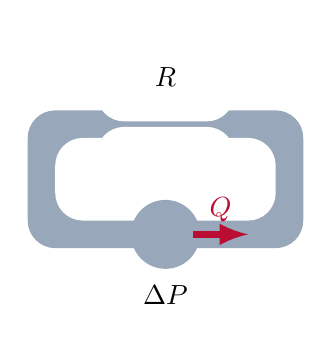
\begin{tikzpicture}[scale=0.7]%
  \scalebox{1}%
  {%
  \def\h{2.5}%
  \def\fac{0.8}
  \def\zer{0.2}
  %\fill[color=myblue!40,rounded corners=10] (-\h,0) -- (-\h,\h) -- (\h,\h) --(\h,0) ;
  %\fill[color=white,rounded corners=10] (-\fac*\h,\zer*\h) -- (-{\fac*\h},\fac*\h) -- (\fac*\h,\fac*\h) --(\fac*\h,\zer*\h) --(-\fac*\h,\zer*\h) ;
  \fill[color=myblue!40,rounded corners=10]  (-\h,0) rectangle (\h,\h) ;
  \fill[color=white,rounded corners=10] (-\fac*\h,\zer*\h) rectangle (\fac*\h,\fac*\h) ;
  \fill[color=myblue!40] (0,\zer/2.0*\h) circle(\h/4);
  
  \fill[color=white,rounded corners=10] (-\h/2,0.5*\fac*\h) rectangle (\h/2,1.1*\fac*\h) ;
  \fill[color=white,rounded corners=10] (-\h/2,1.1*\fac*\h+0.2*\zer*\h) rectangle (\h/2,2*\fac*\h) ;
  
  \node[below=10pt] at (0,0) {$\Delta P$};
  \node[above=5pt] at (0,\h) {$R$};
  \draw[-latex, line width=2.5, color=qred] (0.5,\zer/2.0*\h) -- (1.5,\zer/2.0*\h) node[above, midway]{$Q$};

  }%
\end{tikzpicture}%
\captionof*{figure}{\textit{Fluid is driven through the resistor by a difference in pressure (e.g. from a pump). The flow rate is the same everywhere in the pipe (continuity).}}%

\end{columns}

}

%%%%%%%%%%%%%%%%%%%%%%%%%%%%%%
\twocolframesf{Kirchhoff's rules}
{
\begin{itemize}
\item \textbf{Charge conservation:}
\begin{itemize}
\item Charges cannot just appear or disappear from a circuit, they have to go somewhere (there is nowhere for water to enter or leave a closed system).
\end{itemize}
\item \textbf{Energy conservation:}
\begin{itemize}
\item If a charge moves around a loop in a circuit, its energy must not change (the water does not flow faster and faster in a closed system).
\end{itemize}
\end{itemize}
}
{
\capfig{0.6}{figures/Circuits/fountain}{A garden fountain is a closed system. There are multiple paths for the water to go down (resistors in parallel). Since there is no paddle wheel, what is the water’s kinetic energy being converted to?}
}

%%%%%%%%%%%%%%%%%%%%%%%%%%%%%%




\section{Kirchoff's Laws}
\label{sec:kirchoffslaws}
\title{Kirchoff's Laws}


%%%%%%%%%%%%%%%%%%%%%%%%%
\begin{frame}
\titlepage
\thispagestyle{empty}
\end{frame}




%%%%%%%%%%%%%%%%%%%%%%%%%%%%
\subsection{Kirchoff's rules}
\label{subsec:kirchoffsrules}
\twocolframe{Kirchhoff's rules}
{
\begin{itemize}
\item \textbf{Junction rule} (charge):
\begin{itemize}
\item The sum of the currents coming into a junction
must equal the sum of the currents coming out of a
junction:
\begin{align*}
\text{incoming current} &= \text{outgoing current}\\
I_1+I_2+I_4 &= I_3+I_5
\end{align*}
\end{itemize}
\item \textbf{Loop rule} (energy):
\begin{itemize}
\item The sum of the potential differences in any closed loop must be zero:
\begin{align*}
V_1+V_2+V_3+\Delta V=0
\end{align*}
\end{itemize}
\end{itemize}
}
{
\vspace{-0.5cm}
\centering
 \begin{circuitikz}[scale=0.7]%
\scalebox{1}%
{%
\def\h{2.5}%
\draw (45:\h) [short,i=$I_1$] to (0,0);%
\draw (95:\h) [short,i=$I_2$] to (0,0);%
\draw (0,0) [short,i=$I_3$] to (145:\h);%\\
\draw (210:\h) [short,i=$I_4$] to (0,0);%
\draw (0,0) [short,i=$I_5$] to (290:\h);%
\fill (0,0) circle(2pt);
}%
\end{circuitikz}%
\captionof*{figure}{\textit{The junction rule.}}%

 \begin{circuitikz}[scale=0.7]%
\scalebox{1}%
{%
\def\h{1.4}%
\draw (3*\h,0) [battery1=$\Delta V$,-*] to (-3*\h,0);%
\draw (-3*\h,0) [short,-*] to (-3*\h,\h);%
\draw (-3*\h,\h) [R,l^={$V_1=IR_1$},-*] to (-1*\h,\h);
\draw (-1*\h,\h) [R,l^={$V_2=IR_2$},-*] to (1*\h,\h);
\draw (1*\h,\h) [R,l^={$V_3=IR_3$},-*] to (3*\h,\h) ;%
\draw (3*\h,\h) [short,-*] to (3*\h,0);%
}%
\end{circuitikz}%
\captionof*{figure}{\textit{The loop rule.}}%

}


%%%%%%%%%%%%%%%%%%%%%%%%%%%%%%
\subsection{Using Kirchoff's laws}
\twocolframe{Using Kirchhoff's Laws}
{
Getting started
\begin{enumerate}
\item Make a well-labeled diagram.
\item Identify the junctions.
\item Identify the loops.
\end{enumerate}
}
{
\begin{circuitikz}[scale=0.7]
\scalebox{1}
{
\def\h{2}
\def\L{4}

 \draw (-\L,0) node[below] {f}   [battery1,l_={$V_1=\SI{24}{V}$},*-*] to (0,0);
 \draw (-\L,0) to [short,-*] (-\L,\L) node[above] {a}
       to [R,l_={$R_1=\SI{3}{\Omega}$},-*] (0,\L) node[above] {b}
       to [R,l_={$R_2=\SI{3}{\Omega}$}] (0,0) node[below] {e} ;
 \draw (0,0)  [battery1,l_={$V_2=\SI{29}{V}$},*-,invert] to (\L,0) node[below] {d};
 \draw (\L,0) to [R,l^={$R_4=\SI{4}{\Omega}$},-*]  (\L,\L) node[above] {c}
       to [R,l^={$R_3=\SI{3}{\Omega}$}] (0,\L);             

}
\end{circuitikz}%
\captionof*{figure}{\textit{We would like to know all of the currents in this circuit.}}%
}




%%%%%%%%%%%%%%%%%%%%%%%%%%%%%%



%%%%%%%%%%%%%%%%%%%%%%%%%%%%%%

\twocolframe{Using Kirchhoff's Laws}
{
\begin{enumerate}
\item Draw a good diagram with nodes labeled.
\item<2-> Draw ``battery arrows'' from $-$ to $+$.
\item<3-> Make a \textbf{consistent} \emph{guess} for currents.
\only<4-9>{:
\begin{itemize}
\item Start \textit{anywhere} and keep introducing a new current each time you hit a junction.
\end{itemize}
}
\item<10-> Write the Junction Rule (once per junction, up to $N-1$ for $N$ junctions):
\begin{align*}
\boxed{I_1=I_2+I_3}
\end{align*}
Expect 3 unknowns, so need 2 more equations... The loop equations!
\end{enumerate}

}
{
\begin{circuitikz}[scale=0.75]
\scalebox{1}
{
\def\h{2}
\def\L{4}

 \draw (-\L,0) node[below] {f}   [battery1,l_={$V_1=\SI{24}{V}$},*-*] to (0,0);
 \draw (-\L,0) to [short,-*] (-\L,\L) node[above] {a}
       to [R,l_={$R_1=\SI{3}{\Omega}$},-*] (0,\L) node[above] {b}
       to [R,l_={$R_2=\SI{3}{\Omega}$}] (0,0) node[below] {e} ;
 \draw (0,0)  [battery1,l_={$V_2=\SI{29}{V}$},*-,invert] to (\L,0) node[below] {d};
 \draw (\L,0) to [R,l^={$R_4=\SI{4}{\Omega}$},-*]  (\L,\L) node[above] {c}
       to [R,l^={$R_3=\SI{3}{\Omega}$}] (0,\L);             
\only<2->{
 \draw [-latex,color=qred,line width = 4] (-0.4*\L,\h/3+0.2)-- +(-1,0);
 \draw [-latex,color=qred,line width = 4] (0.4*\L,\h/3+0.2)-- +(1,0);
 }

 \only<4->{
 \fill[color=qred] (-\L,0) circle(0.1);
 \draw[-latex,color=qblue,line width = 2] (-\L,0.75*\h)--+(0,1) node[midway,left]{$I_1$};
 } 
 \only<5->{
 \draw[-latex,color=qblue,line width = 2] (-0.95*\L,2*\h)--+(1,0) node[midway,above]{$I_1$};
 \draw[-latex,color=qblue,line width = 2] (-0.3*\L,2*\h)--+(1,0) node[midway,above]{$I_1$};
 \fill[color=qred] (0,2*\h) circle(0.1);
 } 
 \only<6->{
 \draw[-latex,color=qblue,line width = 2] (0.07*\L,2*\h)--+(1,0) node[midway,above]{$I_2$};
  \draw[-latex,color=qblue,line width = 2] (0,1.9*\h)--+(0,-1) node[midway,left]{$I_3$};
 }
 \only<7->{
  \draw[-latex,color=qblue,line width = 2] (0.7*\L,2*\h)--+(1,0) node[midway,above]{$I_2$};
  \draw[-latex,color=qblue,line width = 2] (\L,1.9*\h)--+(0,-1) node[midway,right]{$I_2$};
  \draw[-latex,color=qblue,line width = 2] (\L,0.6*\h)--+(0,-1) node[midway,right]{$I_2$};
  \draw[-latex,color=qblue,line width = 2] (0.95*\L,0)--+(-1,0) node[midway,above]{$I_2$};
  \draw[-latex,color=qblue,line width = 2] (0.3*\L,0)--+(-1,0) node[midway,above]{$I_2$};
 }
 \only<8->{
  \draw[-latex,color=qblue,line width = 2] (0,0.6*\h)--+(0,-1) node[midway,left]{$I_3$};
  \fill[color=qred] (0,0) circle(0.1);
 }
  \only<9->{
  \draw[-latex,color=qblue,line width = 2] (-0.09*\L,0)--+(-1,0) node[midway,above]{$I_1$};
  \draw[-latex,color=qblue,line width = 2] (-0.7*\L,0)--+(-1,0) node[midway,above]{$I_1$};
 }
}
\end{circuitikz}%
\captionof*{figure}{\textit{We want to know all current in this circuit diagram.}}%
}


%%%%%%%%%%%%%%%%%%%%%%%%%%%%%%
\twocolframe{The loop equations}
{
\begin{itemize}
\item \textbf{Important}: \textit{You choose} which way to “walk” around the loop. It’s completely arbitrary. Two rules:
\begin{enumerate}
\item When you encounter a \textbf{\textcolor{qred}{battery arrow: Add the voltage}} if you walk in the same direction as the arrow, subtract otherwise.
\item  When you encounter a \textbf{\textcolor{qblue}{resistor: Subtract the voltage}} across the resistor if you walk in the same direction as the current, add otherwise
\end{enumerate}
\item Across a closed loop, the voltage must be zero.
\end{itemize}

}
{
\begin{circuitikz}[scale=0.75]
\scalebox{1}
{
\def\h{2}
\def\L{4}

 \draw (-\L,0) node[below] {f}   [battery1,l_={$V_1=\SI{24}{V}$},*-*] to (0,0);
 \draw (-\L,0) to [short,-*] (-\L,\L) node[above] {a}
       to [R,l_={$R_1=\SI{3}{\Omega}$},-*] (0,\L) node[above] {b}
       to [R,l_={$R_2=\SI{3}{\Omega}$}] (0,0) node[below] {e} ;
 \draw (0,0)  [battery1,l_={$V_2=\SI{29}{V}$},*-,invert] to (\L,0) node[below] {d};
 \draw (\L,0) to [R,l^={$R_4=\SI{4}{\Omega}$},-*]  (\L,\L) node[above] {c}
       to [R,l^={$R_3=\SI{3}{\Omega}$}] (0,\L);             

 \draw [-latex,color=qred,line width = 4] (-0.4*\L,\h/3)-- +(-1,0);
 \draw [-latex,color=qred,line width = 4] (0.4*\L,\h/3)-- +(1,0);
 


 \draw[-latex,color=qblue,line width = 2] (-\L,0.75*\h)--+(0,1) node[midway,left]{$I_1$};
 \draw[-latex,color=qblue,line width = 2] (-0.3*\L,2*\h)--+(1,0) node[midway,above]{$I_1$};
 \draw[-latex,color=qblue,line width = 2] (-0.09*\L,0)--+(-1,0) node[midway,above]{$I_1$};

 \draw[-latex,color=qblue,line width = 2] (0.07*\L,2*\h)--+(1,0) node[midway,above]{$I_2$};
  \draw[-latex,color=qblue,line width = 2] (\L,1.9*\h)--+(0,-1) node[midway,right]{$I_2$};
  \draw[-latex,color=qblue,line width = 2] (0.3*\L,0)--+(-1,0) node[midway,above]{$I_2$};

  \draw[-latex,color=qblue,line width = 2] (0,1.9*\h)--+(0,-1) node[midway,right]{$I_3$};
  \draw[-latex,color=qblue,line width = 2] (0,0.6*\h)--+(0,-1) node[midway,left]{$I_3$}; 
}
\end{circuitikz}%
\captionof*{figure}{\textit{Circuit diagram with everything well-labeled.}}%
}


%%%%%%%%%%%%%%%%%%%%%%%%%%%%%%
%%%%%%%%%%%%%%%%%%%%%%%%%%%%%%%%%%%





\section{Solving Circuits}
\label{sec:solvingcircuits}
\title{Solving Circuits}


%%%%%%%%%%%%%%%%%%%%%%%%%
\begin{frame}
\titlepage
\thispagestyle{empty}
\end{frame}





%%%%%%%%%%%%%%%%%%%%%%%%%%%%%%%%%
\subsection{Loop equations}
\label{subsec:loopequations}
\twocolframe{The loop equations}
{

\begin{itemize}
\item[$\rightarrow$] Consider loop $abcdefa$:
\only<2>{
\item(ab): with current, $I_1$ through resistor $R_1$: \textcolor{qred}{$-R_1I_1 \rightarrow -3I_1$}
}
\only<3>{ 
\item(bc): with current, $I_2$ through resistor $R_3$: \textcolor{qred}{$-R_3I_2 \rightarrow -3I_2$}
}
\only<4>{ 
\item(cd): with current, $I_2$ through resistor $R_4$: \textcolor{qred}{$-R_3I_2 \rightarrow -4I_2$}
}
\only<5>{ 
\item(de): \textit{against} battery arrow: \textcolor{qred}{$-V_2 \rightarrow -29$}
}
\only<6>{ 
\item(ef): with battery arrow: \textcolor{qred}{$+V_1 \rightarrow +24$}
}
\only<7>{ 
\item(fa): no battery or resistor, so no voltage change. Back to starting point: \textcolor{qred}{$=0$}
}
\only<8>{
\item We now have a second equation (recall that there are 3 unknowns). We need one more loop equation. 
}

\end{itemize}

}
{
\begin{circuitikz}[scale=0.7]
\scalebox{1}
{
\def\h{2}
\def\L{4}

\only<1,2,8>{
\draw[color=qred!50, line width=6,-latex] (-\L,2*\h) -- (0,2*\h) node[midway,above] {\reflectbox{
\includegraphics[scale=.4]{figures/Circuits/girl}}};
}
\only<1,3,8>{
\draw[color=qred!50, line width=6,-latex] (0,2*\h) -- (\L,2*\h)  node[midway,above] {\reflectbox{
\includegraphics[scale=.4]{figures/Circuits/girl}}};
}
\only<1,4,8>{
\draw[color=qred!50, line width=6,-latex] (\L,2*\h) -- (\L,0) node[rotate=-90,midway,above] {\reflectbox{
\includegraphics[scale=.4]{figures/Circuits/girl}}};
}
\only<1,5,8>{
\draw[color=qred!50, line width=6,-latex] (\L,0) -- (0,0)node[rotate=-180,midway,above] {\reflectbox{
\includegraphics[scale=.4]{figures/Circuits/girl}}};
}
\only<1,6,8>{
\draw[color=qred!50, line width=6,-latex] (0,0) -- (-\L,0)node[rotate=-180,midway,above] {\reflectbox{
\includegraphics[scale=.4]{figures/Circuits/girl}}};
}
\only<1,7,8>{
\draw[color=qred!50, line width=6,-latex] (-\L,0) -- (-\L,2*\h)node[rotate=-270,midway,above] {\reflectbox{
\includegraphics[scale=.4]{figures/Circuits/girl}}};
}

 \draw (-\L,0) node[below] {f}   [battery1,l_={$V_1=\SI{24}{V}$},*-*] to (0,0);
 \draw (-\L,0) to [short,-*] (-\L,\L) node[above] {a}
       to [R,l_={$R_1=\SI{3}{\Omega}$},-*] (0,\L) node[above] {b}
       to [R,l_={$R_2=\SI{3}{\Omega}$}] (0,0) node[below] {e} ;
 \draw (0,0)  [battery1,l_={$V_2=\SI{29}{V}$},*-,invert] to (\L,0) node[below] {d};
 \draw (\L,0) to [R,l^={$R_4=\SI{4}{\Omega}$},-*]  (\L,\L) node[above] {c}
       to [R,l^={$R_3=\SI{3}{\Omega}$}] (0,\L);             

 \draw [-latex,color=qred,line width = 4] (-0.4*\L,\h/3+0.2)-- +(-1,0);
 \draw [-latex,color=qred,line width = 4] (0.4*\L,\h/3+0.2)-- +(1,0);
 


 \draw[-latex,color=qblue,line width = 2] (-\L,0.75*\h)--+(0,1) node[midway,left]{$I_1$};
 \draw[-latex,color=qblue,line width = 2] (-0.3*\L,2*\h)--+(1,0) node[midway,above]{$I_1$};
 \draw[-latex,color=qblue,line width = 2] (-0.09*\L,0)--+(-1,0) node[midway,above]{$I_1$};

 \draw[-latex,color=qblue,line width = 2] (0.07*\L,2*\h)--+(1,0) node[midway,above]{$I_2$};
  \draw[-latex,color=qblue,line width = 2] (\L,1.9*\h)--+(0,-1) node[midway,right]{$I_2$};
  \draw[-latex,color=qblue,line width = 2] (0.3*\L,0)--+(-1,0) node[midway,above]{$I_2$};

  \draw[-latex,color=qblue,line width = 2] (0,1.9*\h)--+(0,-1) node[midway,right]{$I_3$};
  \draw[-latex,color=qblue,line width = 2] (0,0.6*\h)--+(0,-1) node[midway,left]{$I_3$}; 
}
\end{circuitikz}%
\captionof*{figure}{\textit{Going around loop $(abcdefa)$.}}%
\only<2>{
Equation for loop ($abcdefa$):
\begin{align*}
 \textcolor{qred}{-3I_1}\dots
\end{align*}
}
\only<3>{
Equation for loop ($abcdefa$):
\begin{align*}
 -3I_1\textcolor{qred}{\;-3I_2}\dots
\end{align*}
}
\only<4>{
Equation for loop ($abcdefa$):
\begin{align*}
 -3I_1-3I_2\textcolor{qred}{\;-4I_2}\dots
\end{align*}
}
\only<5>{
Equation for loop ($abcdefa$):
\begin{align*}
 -3I_1-3I_2-4I_2\textcolor{qred}{\;-29}\dots
\end{align*}
}
\only<6>{
Equation for loop ($abcdefa$):
\begin{align*}
 -3I_1-3I_2-4I_2-29\textcolor{qred}{\;+24}\dots
\end{align*}
}
\only<7>{
Equation for loop ($abcdefa$):
\begin{align*}
 -3I_1-3I_2-4I_2-29+24\textcolor{qred}{\;=0}
\end{align*}
}
\only<8>{
Equation for loop ($abcdefa$):
\begin{align*}
\therefore -3I_1-3I_2-4I_2-29+24=0
\end{align*}
}

}





%%%%%%%%%%%%%%%%%%%%%%%%%%%%%%
\twocolframe{The loop equations}
{
\begin{itemize}
\item Choose loop $bcdeb$:
\begin{itemize}
\item (bc): $-R_3I_2 \rightarrow -3I_2$ (with current through resistor)
\item (cd): $-R_4I_2 \rightarrow -4I_2$ (with current through resistor)
\item (de): $-V_2 \rightarrow -29$ (\textit{against} battery arrow)
\item (eb): $+R_2I_3 \rightarrow +3I_3$ (\textit{against} current through resistor)
\end{itemize}
\end{itemize}
}
{
\begin{circuitikz}[scale=0.75]
\scalebox{1}
{
\def\h{2}
\def\L{4}

\draw[color=qred!50, line width=6,-latex] (0,2*\h) -- (\L,2*\h);
\draw[color=qred!50, line width=6,-latex] (\L,2*\h) -- (\L,0);
\draw[color=qred!50, line width=6,-latex] (\L,0) -- (0,0);
\draw[color=qred!50, line width=6,-latex] (0,0) -- (0,2*\h);

 \draw (-\L,0) node[below] {f}   [battery1,l_={$V_1=\SI{24}{V}$},*-*] to (0,0);
 \draw (-\L,0) to [short,-*] (-\L,\L) node[above] {a}
       to [R,l_={$R_1=\SI{3}{\Omega}$},-*] (0,\L) node[above] {b}
       to [R,l_={$R_2=\SI{3}{\Omega}$}] (0,0) node[below] {e} ;
 \draw (0,0)  [battery1,l_={$V_2=\SI{29}{V}$},*-,invert] to (\L,0) node[below] {d};
 \draw (\L,0) to [R,l^={$R_4=\SI{4}{\Omega}$},-*]  (\L,\L) node[above] {c}
       to [R,l^={$R_3=\SI{3}{\Omega}$}] (0,\L);             

 \draw [-latex,color=qred,line width = 4] (-0.4*\L,\h/3+0.2)-- +(-1,0);
 \draw [-latex,color=qred,line width = 4] (0.4*\L,\h/3+0.2)-- +(1,0);
 
 \draw[-latex,color=qblue,line width = 2] (-\L,0.75*\h)--+(0,1) node[midway,left]{$I_1$};
 \draw[-latex,color=qblue,line width = 2] (-0.3*\L,2*\h)--+(1,0) node[midway,above]{$I_1$};
 \draw[-latex,color=qblue,line width = 2] (-0.09*\L,0)--+(-1,0) node[midway,above]{$I_1$};

 \draw[-latex,color=qblue,line width = 2] (0.07*\L,2*\h)--+(1,0) node[midway,above]{$I_2$};
  \draw[-latex,color=qblue,line width = 2] (\L,1.9*\h)--+(0,-1) node[midway,right]{$I_2$};
  \draw[-latex,color=qblue,line width = 2] (0.3*\L,0)--+(-1,0) node[midway,above]{$I_2$};

  \draw[-latex,color=qblue,line width = 2] (0,1.9*\h)--+(0,-1) node[midway,right]{$I_3$};
  \draw[-latex,color=qblue,line width = 2] (0,0.6*\h)--+(0,-1) node[midway,left]{$I_3$}; 
}
\end{circuitikz}%
\captionof*{figure}{\textit{Circuit diagram with loop $(bcdeb)$ highlighted.}}%

Equation for loop ($bcdeb$):
\begin{align*}
\therefore -3I_2-4I_2-29+3I_3=0
\end{align*}
}



%%%%%%%%%%%%%%%%%%%%%%%%%%%%%%
\subsection{Solving circuits using loop equations}
\label{subsec:solvingcircuitsusingloopequations}
\twocolframe{Solving the circuit}
{
\begin{itemize}
\item We now have 3 equations and 3 unknowns, allowing us to determine all of the currents.
\begin{align*}
I_2+I_3&=I_1 &\text{(Junction rule)}\\
-3I_1-3I_2-4I_2-29+24&=0 &\text{(Loop abcdefa)}\\
-3I_2-4I_2-29+3I_3&=0 &\text{(Loop bcdeb)}
\end{align*}
\item The system of linear equations is easier to handle if you don't include the units (so make sure everything is in SI units!).
\end{itemize}
}
{
\begin{circuitikz}[scale=0.7]
\scalebox{1}
{
\def\h{2}
\def\L{4}

 \draw (-\L,0) node[below] {f}   [battery1,l_={$V_1=\SI{24}{V}$},*-*] to (0,0);
 \draw (-\L,0) to [short,-*] (-\L,\L) node[above] {a}
       to [R,l_={$R_1=\SI{3}{\Omega}$},-*] (0,\L) node[above] {b}
       to [R,l_={$R_2=\SI{3}{\Omega}$}] (0,0) node[below] {e} ;
 \draw (0,0)  [battery1,l_={$V_2=\SI{29}{V}$},*-,invert] to (\L,0) node[below] {d};
 \draw (\L,0) to [R,l^={$R_4=\SI{4}{\Omega}$},-*]  (\L,\L) node[above] {c}
       to [R,l^={$R_3=\SI{3}{\Omega}$}] (0,\L);             

 \draw [-latex,color=qred,line width = 4] (-0.4*\L,\h/3+0.2)-- +(-1,0);
 \draw [-latex,color=qred,line width = 4] (0.4*\L,\h/3+0.2)-- +(1,0);
 
 \draw[-latex,color=qblue,line width = 2] (-\L,0.75*\h)--+(0,1) node[midway,left]{$I_1$};
 \draw[-latex,color=qblue,line width = 2] (-0.3*\L,2*\h)--+(1,0) node[midway,above]{$I_1$};
 \draw[-latex,color=qblue,line width = 2] (-0.09*\L,0)--+(-1,0) node[midway,above]{$I_1$};

 \draw[-latex,color=qblue,line width = 2] (0.07*\L,2*\h)--+(1,0) node[midway,above]{$I_2$};
  \draw[-latex,color=qblue,line width = 2] (\L,1.9*\h)--+(0,-1) node[midway,right]{$I_2$};
  \draw[-latex,color=qblue,line width = 2] (0.3*\L,0)--+(-1,0) node[midway,above]{$I_2$};

  \draw[-latex,color=qblue,line width = 2] (0,1.9*\h)--+(0,-1) node[midway,right]{$I_3$};
  \draw[-latex,color=qblue,line width = 2] (0,0.6*\h)--+(0,-1) node[midway,left]{$I_3$}; 
}
\end{circuitikz}%
\captionof*{figure}{\textit{Well-labeled circuit diagram.}}%
}


%%%%%%%%%%%%%%%%%%%%%%%%%%%%%%
\subsection{Solving a ciruit - foolproof method!}
\label{subsec:solcingacircuitfoolproofmethod}
\twocolframesf{Solving a circuit - Foolproof method!}
{
\begin{enumerate}
\item Make a good diagram.
\item Simplify resistors that can be combined.
\item Draw ``battery arrows'', from $-$ to $+$ (small slide to big side).
\item Guess currents in a consistent manner (start somewhere and proceed).
\item Write the junction rule equations (once per junction).
\item Write the loop equations.
\item Solve $N$ equations for $N$ unknown currents.
\end{enumerate}
}
{
\vspace{-1.75cm}
\vspace{-1cm}
\begin{exampleblock}{Direction of current(s)}
It is possible that you find negative values for the current(s). In that case, \textbf{first, solve for all of the other currents}. Then, \textit{at the very end}, reverse the arrows in the diagram since you guessed the direction wrong (but in a consistent way!).
\end{exampleblock}
}


%%%%%%%%%%%%%%%%%%%%%%%%%%%%%%





%%%%%%%%%%%%%%%%%%%%%%%%%%%%%%%


\subsection{The galvanometer}
\label{subsec:thegalvanometer}
\twocolframe{The galvanometer}
{
\begin{itemize}
\item As we will learn, a wire that carries a current will feel a force if placed in a magnetic field.
\item A galvanometer is a very sensitive device for measuring current.
\item Typically, they measure currents of order micro amperes.
\item Can obviously use to measure current.
\item Can also use to measure voltage.
\end{itemize}
}
{
\capfig{1}{figures/Circuits/galvanometer}{A galvanometer}
}

%%%%%%%%%%%%%%%%%%%%%%%%%%%%%%
\subsection{Measuring current}
\label{subsec:measuringcurrent}
\twocolframe{Measuring current}
{
\begin{itemize}
\only<1>{
\item Based on using a galvanometer:
\begin{itemize}
\item[$\rightarrow$] Need to have a very small current through the galvanometer
\end{itemize}
\item An \textbf{ammeter} measures currents, even potentially large ones.
\item We thus add a resistor in \textbf{parallel} with a galvanometer to create an ammeter.
\item This is called a \textit{shunt} resistor.
}
\only<2>{
\item We know the current through the galvanometer and the value of all resistors.
The total current is:
\begin{align*}
I=I_G+I_s
\end{align*}
\item Both resistors have the same potential difference:
\begin{align*}
R_GI_G=R_sI_s
\end{align*}
\item The total current, in terms of $I_G$, is thus:
\begin{align*}
I=I_G+I_s=I_G\left( 1 + \frac{R_G}{R_s}\right)
\end{align*}
}
\end{itemize}
}
{
\centering
 \begin{circuitikz}[scale=0.7]%
\scalebox{1}%
{%
\def\h{1.5}%
\draw (-1.5*\h,0) [short,*-] to (0,0);

\draw (0,0) [short] to (0,\h);
\draw (0,\h) [rmeter,t=G] to (2*\h,\h);
\draw (2*\h,\h) [short] to (2*\h,0);

\draw (0,0) [short] to (0,-\h);
\draw (0,-\h) [R=$R_s$] to (2*\h,-\h);
\draw (2*\h,-\h) [short] to (2*\h,0);

\draw (2*\h,0) [short,-*] to (3.5*\h,0);

\draw[dotted, color=qblue!70, line width=2] (-0.3*\h ,-1.3*\h) rectangle(2.3*\h ,1.6*\h) node [above=7pt,left] {Ammeter};


\draw[color=qred, line width=1pt, -latex] (-1.7,0) -- +(1,0) node[midway, above] {$I$};
\draw[color=qred, line width=1pt, -latex] (3.9,0) -- +(1,0) node[midway, above] {$I$};
\draw[color=qred, line width=1pt, -latex] (0,0.2) -- +(0,1) node[midway, right] {$I_G$};
\draw[color=qred, line width=1pt, -latex] (0,-0.2) -- +(0,-1) node[midway, right] {$I_s$};
 
 }%
\end{circuitikz}%
\captionof*{figure}{\textit{An ammeter made using a galvanometer and a (small) shunt resistor. Most of the current goes through the shunt. An ammeter is connected in series and has a very low resistance.}}%

}

%%%%%%%%%%%%%%%%%%%%%%%%%%%%%%
\subsection{Measuring Voltage}
\twocolframe{Measuring Voltage}
{
\begin{itemize}
\item Again, we need a small current through the galvanometer, but would like to measure a large potential difference.
\item We place a large resistor in \textbf{series} with the galvanometer.
\item Both see the same current, so if R is large it will have the biggest potential difference.
\begin{align*}
\Delta V = I_G(R + R_G)
\end{align*}
\end{itemize}
}
{
\centering
 \begin{circuitikz}[scale=0.7]%
\scalebox{1}%
{%
\def\h{1.5}%
\draw (-1.0*\h,0) [short,*-] to (0,0);
\draw (0,0) [R=$R$] to (2*\h,0);
\draw (2*\h,0) [rmeter,t=G] to (3.0*\h,0);
\draw (3.0*\h,0) [short,-*] to (4.0*\h,0);

\draw[dotted, color=qblue!70, line width=2] (-0.2*\h,-0.7*\h) rectangle(3.2*\h ,1*\h) node [above=7pt,left] {Voltmeter};

\draw[color=qred, line width=1pt, -latex] (-1.4,0) -- +(1,0) node[midway, above] {$I_G$};
\draw[latex-latex, line width=1.5pt] (-\h,-\h) -- (4*\h,-\h) node[midway,below] {$\Delta V$};
}
\end{circuitikz}%
\captionof*{figure}{\textit{A voltmeter made using a galvanometer and a (large) resistor in series. Most of the voltage drop happens across the large resistor, $R$. A voltmeter is connected in parallel and has a very large resistance.}}%
}

%%%%%%%%%%%%%%%%%%%%%%%%%%%%%%
\subsection{The multimeter}
\label{subsec:themultimeter}
\twocolframesf{The multimeter}
{
\begin{itemize}
\item Can measure current, voltage and resistance.
\item The knob chooses the value of the resistor and its configuration.
\item To measure resistance, the device has an internal voltage source; it then measures the current across a resistor connected across it leads (the resistor cannot be connected to anything else).
\end{itemize}
}
{
\capfig{0.9}{figures/Circuits/multimeter}{https://www.amazon.ca/Digital-Multimeter-Voltmeter-Ohmmeter-Detachable/dp/B08K3G2GRF}
}


\subsection{RC circuits}
\label{subsec:rccircuits}
\twocolframesf{RC Circuits}
{
\begin{itemize}
\item Consider a circuit with a resistor and a capacitor:
\begin{itemize}
\item Current cannot flow through a capacitor.
\item Capacitor charges up with time, until current is zero.
\item[$\rightarrow$] The current in an RC circuit is not constant!
\end{itemize}
Consider the loop rule (recall $Q=CV$ for a capacitor:
\begin{align*}
\Delta V - IR - \frac{Q}{C} &=0\\
\Delta V - \frac{dQ}{dt}R - \frac{Q}{C} &=0\\
\therefore Q(t) &= C\Delta V\left (1-e^{-\frac{t}{RC}}\right)
\end{align*} 

\end{itemize}

}
{
\vspace{-1cm}
\begin{center}
\begin{circuitikz}
 \draw (0,0) to [short] (0,2)
       to [R=$R$] (2,2)
       to [C=$C$] (4,2)
       to [nos, l_=S] (4,0)
       to [battery1,v^=$\Delta V$] (0,0);        
\end{circuitikz}
\captionof*{figure}{\label{fig:circuits:RCcircuit}\textit{ A simple circuit with a resistor, battery, and capacitor.}} 
\end{center}
When the switch is closed, current decreases exponentially with time:
\begin{align*}
I(t) = \frac{dQ}{dt} = \frac{\Delta V}{R} e^{-\frac{t}{RC}}
\end{align*}
}


%%%%%%%%%%%%%%%%%%%%%%%%%%%%%%%






%%%%%%%%%%%%%%%%%%%%%%%%%%%%%%%%%






%%%%%%%%%%%%%%%%%%%%%%%%%%%%%%%%%%%






%%%%%%%%%%%%%%%%%%%%%%%%%%%%%%%%%%%%%





%%%%%%%%%%%%%%%%%%%%%%%%%%%%%%%%%%%%%%%%




%%%%%%%%%%%%%%%%%%%%%%%%%%%%%%%%%%%%%%%%%%%%



\end{document}
